\section{Choosing the Stopping Criterion Precision} \label{sec:choosing_stopping_criterion_precision}

The standard stopping criterion for gradient descent methods is 
\[\norm{\nabla f(\mathbf{x}^{(k)})}_2 < \varepsilon\]
where \(f\) is the objective function and \(\mathbf{x}^{(k)}\) is the solution vector after the \(k\)th iteration.
This section will try to show the difficulty of choosing a reasonable \(\varepsilon\) for our purposes.
The graphs in this section are all generated by the following parameters:
\begin{itemize}
 \item Objective function: \(T_{\NWA_\gamma}\) with \(\gamma = 10^5\)
 \item Start vector: CENTER
 \item Optimization method: Nesterov's accelerated gradient method
 \item The step size strategy: \texttt{barzilai-borwein}
 \item The stopping criterion: After exactly 500 iterations
\end{itemize}

Because the choice of \(\varepsilon\) can depend on the problem instance,
it is time to introduce more chips to compare results on.
\cref{table:chip_properties} is an overview of the sizes of these instances.
\texttt{Chip1} and \texttt{Chip2} have the same chip area and similar numbers of cells, pins and nets
but differ in the specific way the cells are set up.
\texttt{Chip3} and \texttt{Chip4} are included to see how \(\NWA\) performs on smaller instances.

\begin{table}[ht] 
 \centering
 \begin{tabular}{c c c c c c}
  Instance       & \# Cells & \# Nets   & \# Pins   & Width [\si{\micro\meter}] & Height [\si{\micro\meter}] \\
  \hline
  \texttt{Chip1} & 1,900,000        & 1,900,000 & 5,600,000 & 1300                          & 900 \\
  \texttt{Chip2} & 1,800,000        & 1,800,000 & 5,400,000 & 1300                          & 900 \\
  \texttt{Chip3} & 800,000          & 600,000   & 2,200,000 & 1800                          & 400 \\
  \texttt{Chip4} & 300,000          & 300,000   & 800,000   & 400                           & 200 \\
 \end{tabular}
 \caption{Rounded properties of the newly introduced instances}
 \label{table:chip_properties}
\end{table}


\begin{figure}[ht]
 \centering
 \begin{tikzpicture}
  \begin{groupplot} [
      width=(\textwidth-1cm),
      height=(\textwidth-1cm)/2,
      group style={group size=1 by 1},
      group/xlabels at=edge bottom,
      xlabel=Iteration,
      ylabel=Gradient norm,
      y unit=\si{\micro\meter},
      yticklabel style={/pgf/number format/fixed},
      legend columns=2,
      enlarge x limits={value=0.05, upper},
      xmin=0,
      ymax=0.03,
  ]
   \nextgroupplot
   \addlegendentry{\texttt{Chip1}, X}
   \addplot [red, thick] table [
    x=iteration,
    y expr=\thisrow{NAG_barzilai-borwein_euclidean_norm_X}
   ] {chapters/results/epsilon/convergence_Chip1_by_step_size_strategy_and_dim.data};

   \addlegendentry{\texttt{Chip1}, Y}
   \addplot [red, thick, dashed] table [
    x=iteration,
    y expr=\thisrow{NAG_barzilai-borwein_euclidean_norm_Y},
   ] {chapters/results/epsilon/convergence_Chip1_by_step_size_strategy_and_dim.data};

   \addlegendentry{\texttt{Chip2}, X}
   \addplot [dark_green, thick] table [
    x=iteration,
    y expr=\thisrow{NAG_barzilai-borwein_euclidean_norm_X}
   ] {chapters/results/epsilon/convergence_Chip2.data};

   \addlegendentry{\texttt{Chip2}, Y}
   \addplot [dark_green, thick, dashed] table [
    x=iteration,
    y expr=\thisrow{NAG_barzilai-borwein_euclidean_norm_Y},
   ] {chapters/results/epsilon/convergence_Chip2.data};
   
   \addlegendentry{\texttt{Chip3}, X}
   \addplot [blue, thick] table [
    x=iteration,
    y expr=\thisrow{NAG_barzilai-borwein_euclidean_norm_X},
   ] {chapters/results/epsilon/convergence_Chip3.data};

   \addlegendentry{\texttt{Chip3}, Y}
   \addplot [blue, thick, dashed] table [
    x=iteration,
    y expr=\thisrow{NAG_barzilai-borwein_euclidean_norm_Y},
   ] {chapters/results/epsilon/convergence_Chip3.data};

   \addlegendentry{\texttt{Chip4}, X}
   \addplot [Goldenrod, thick] table [
    x=iteration,
    y expr=\thisrow{NAG_barzilai-borwein_euclidean_norm_X},
   ] {chapters/results/epsilon/convergence_Chip4.data};

   \addlegendentry{\texttt{Chip4}, Y}
   \addplot [Goldenrod, thick, dashed] table [
    x=iteration,
    y expr=\thisrow{NAG_barzilai-borwein_euclidean_norm_Y},
   ] {chapters/results/epsilon/convergence_Chip4.data};
   
   \addlegendentry{0.004\si{\micro\meter}}
   \addplot[black] coordinates {(0,0)};
   
   \draw[black] (axis cs:0,0.004) -- (axis cs:600,0.004);
  \end{groupplot}
 \end{tikzpicture}
 \caption{Gradient norm by iteration depending on the instance} 
 \label{fig:epsilon_convergence_by_chip}
\end{figure} 

The simplest option for choosing \(\varepsilon\) would be using the same value for all instances.
In \cref{fig:epsilon_convergence_by_chip}, the Euclidean norms of the gradients during the optimization processes are graphed.
This time x- and y-direction are considered seperately because when the two optimization processes run in parallel
the stopping criterion cannot depend on both but has to be considered for each of them seperately.
The first clear insight that can be gained by looking at the graph is that,
although it was one of the important aspects of choosing the current paramters,
the gradient norm can still stagnate above zero for some time.
Take a look at the x-direction of \texttt{Chip1} for example:
After the first 100 iterations the gradient norm is decreasing very slowly
and only drops below 0.005\si{\micro\meter} after 400 iterations.
Reaching 0.008\si{\micro\meter} takes about 200 iterations,
reaching 0.006\si{\micro\meter} about 400
and reaching 0.004\si{\micro\meter} more than 500 (in fact around 650).
In other words, small increases in desired precision lead to great increases in runtime.

The second observation is that a single \(\varepsilon\) for all these instances
does not lead to a comparable number of iterations even for similar instances.
Say, for example, that \(\varepsilon\) is set to \(0.004\si{\micro\meter}\) (the value is marked in \cref{fig:epsilon_convergence_by_chip}).
Then \texttt{Chip2} would reach the stopping criterion after roughly 250 iterations for both directions
while \texttt{Chip1} would need more than 500 iterations to reduce the gradient norm of both directions below this value.
This is the case even though \texttt{Chip1} and \texttt{Chip2} are very similar
and the placements profit similarly from an increased number of iterations.
The value of \(\varepsilon\) is supposed to control the compromise of solution quality and runtime
but at least for some values of it the solution quality and runtime differs wildly even for similar chips
which makes this stopping criterion unusable.

It may be possible to scale the gradient norms appropriately so that they all line up
and a single threshold becomes viable
but is unclear how exactly the scaling factor has to be chosen so that the graphs match up
because it is unclear which factors influence the gradient norm in which way.
Therefore we chose to not depend on the gradient norm as a stopping criterion but instead
fix the number of iterations as before.
This way the computation time scales in a predictable way with the instance size
and it avoids that one of the two optimization processes on a chip is terminated
much earlier than the other.

Now the question becomes how many iterations are reasonable when one has to balance solution quality with runtime.
In 
\cref{fig:placement_Chip1_depending_on_max_iterations,fig:placement_Chip2_depending_on_max_iterations,fig:placement_Chip3_depending_on_max_iterations,fig:placement_Chip4_depending_on_max_iterations},
the placement plots after 50, 100 and 200 iterations are shown for each chip.
The corresponding runtimes are recorded in \cref{table:runtime_depending_on_max_iterations}.

\begin{figure}[p]
 \centering

 \begin{subfigure}{.48\textwidth}
  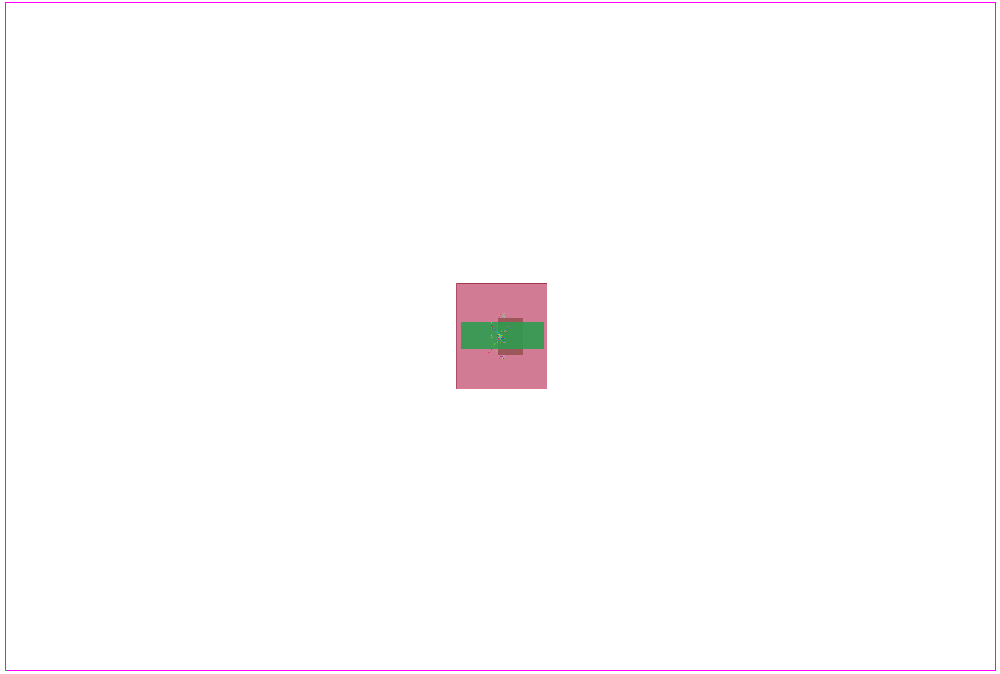
\includegraphics[width=\textwidth]{epsilon/placement_Chip1_50_iterations.png}
  \caption{50 iterations}
 \end{subfigure}
 \hfill
 \begin{subfigure}{.48\textwidth}
  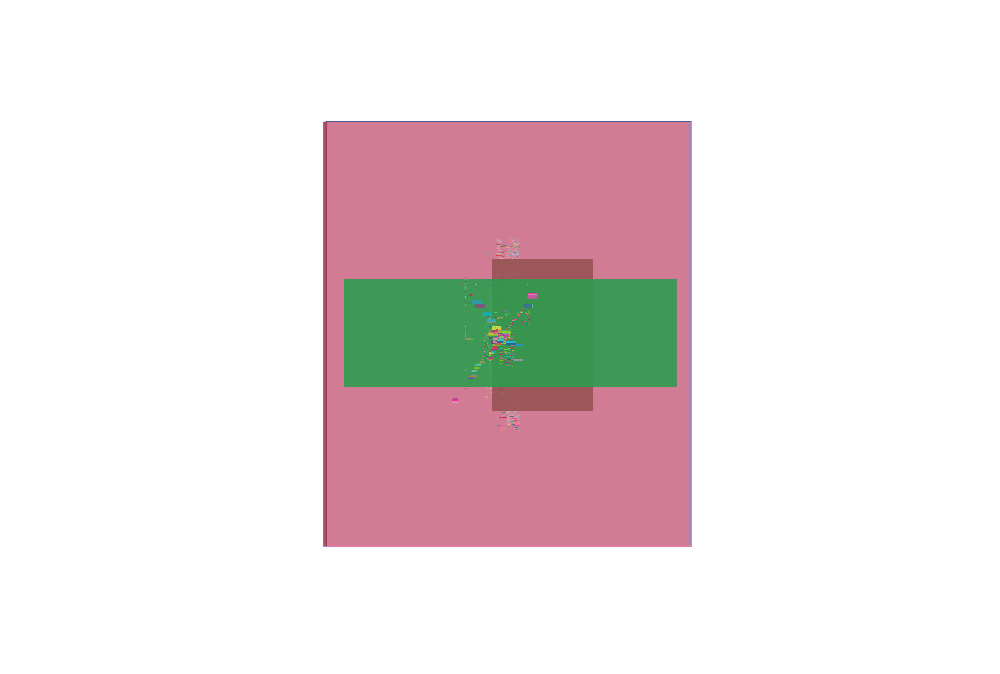
\includegraphics[width=\textwidth, frame]{epsilon/placement_Chip1_50_iterations_zoomed.png}
  \caption{50 iterations, zoomed in on center}
 \end{subfigure}
 
 \bigskip
 
 \begin{subfigure}{.48\textwidth}
  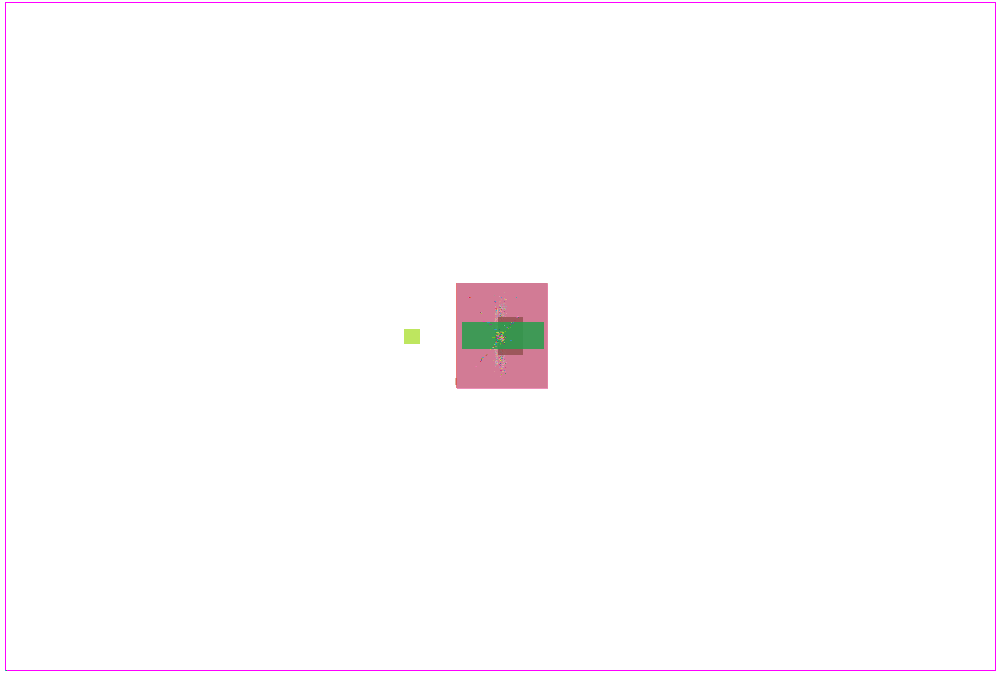
\includegraphics[width=\textwidth]{epsilon/placement_Chip1_100_iterations.png}
  \caption{100 iterations}
 \end{subfigure}
 \hfill
 \begin{subfigure}{.48\textwidth}
  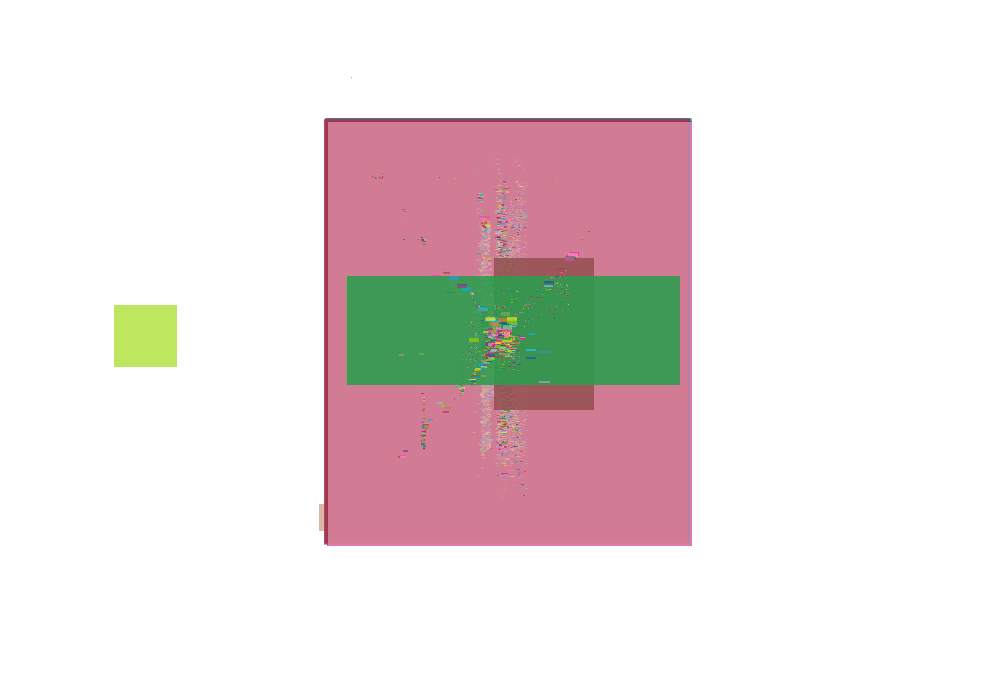
\includegraphics[width=\textwidth, frame]{epsilon/placement_Chip1_100_iterations_zoomed.png}
  \caption{100 iterations, zoomed in on center}
 \end{subfigure}
 
 \bigskip
 
 \begin{subfigure}{.48\textwidth}
  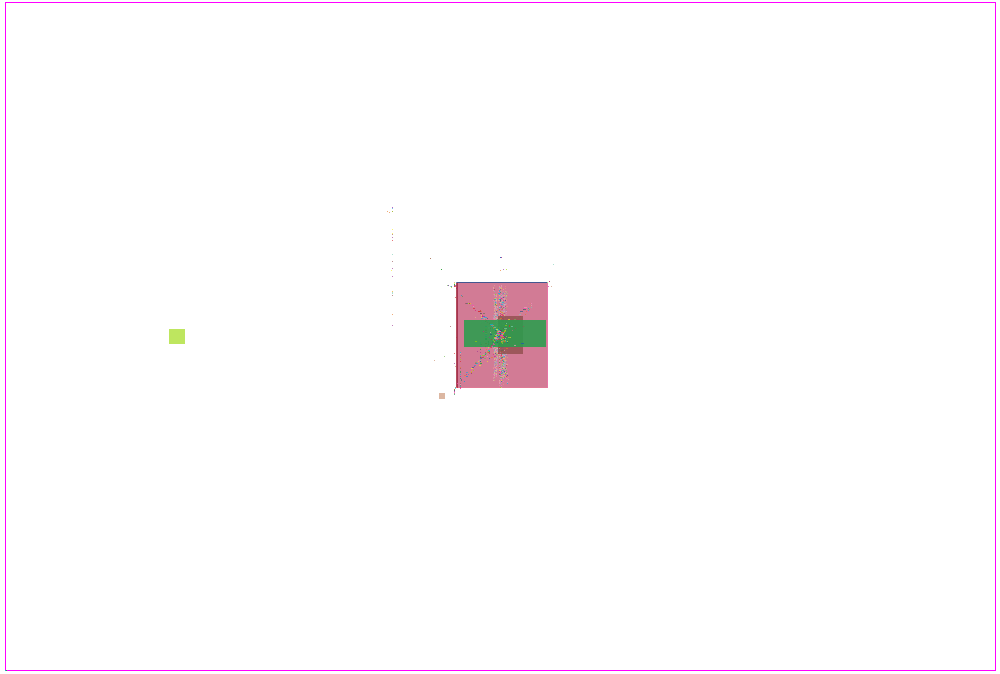
\includegraphics[width=\textwidth]{epsilon/placement_Chip1_200_iterations.png}
  \caption{200 iterations}
 \end{subfigure}
 \hfill
 \begin{subfigure}{.48\textwidth}
  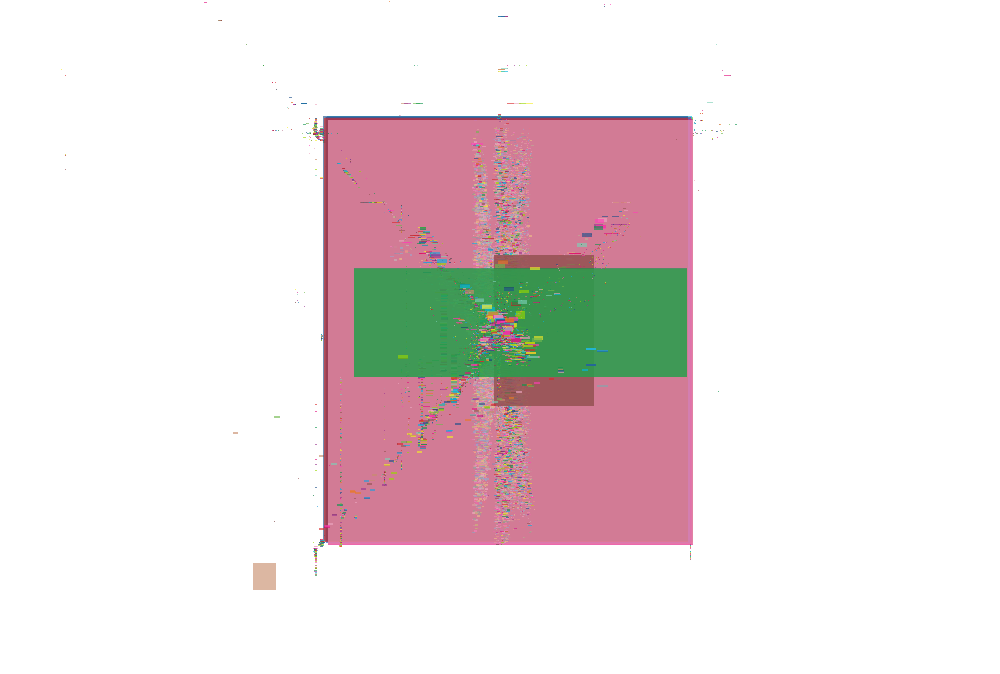
\includegraphics[width=\textwidth, frame]{epsilon/placement_Chip1_200_iterations_zoomed.png}
  \caption{200 iterations, zoomed in on center}
 \end{subfigure}

 \caption{Placement plots after 50, 100 and 200 NAG iterations for \texttt{Chip1}}
 \label{fig:placement_Chip1_depending_on_max_iterations}
\end{figure}

\begin{figure}[p]
 \centering

 \begin{subfigure}{.48\textwidth}
  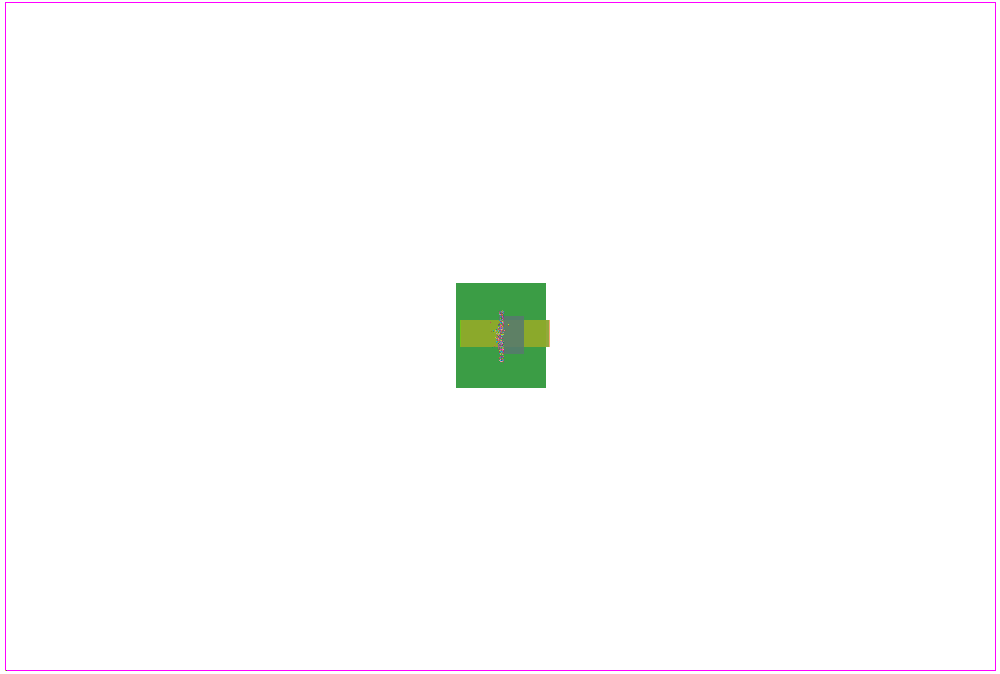
\includegraphics[width=\textwidth]{epsilon/placement_Chip2_50_iterations.png}
  \caption{50 iterations}
 \end{subfigure}
 \hfill
 \begin{subfigure}{.48\textwidth}
  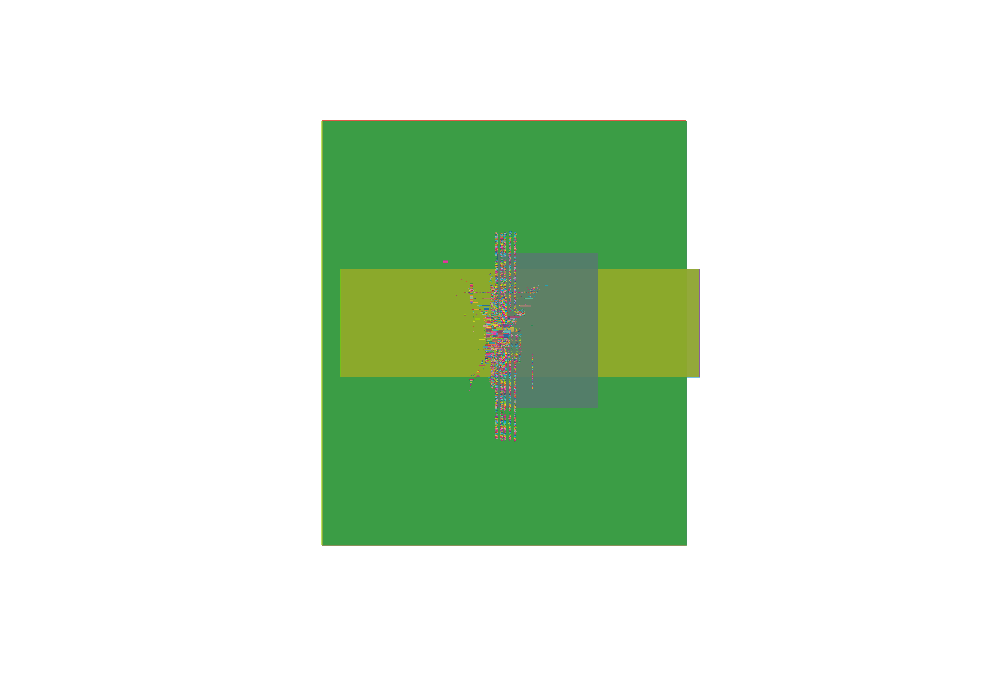
\includegraphics[width=\textwidth, frame]{epsilon/placement_Chip2_50_iterations_zoomed.png}
  \caption{50 iterations, zoomed in on center}
 \end{subfigure}
 
 \bigskip
 
 \begin{subfigure}{.48\textwidth}
  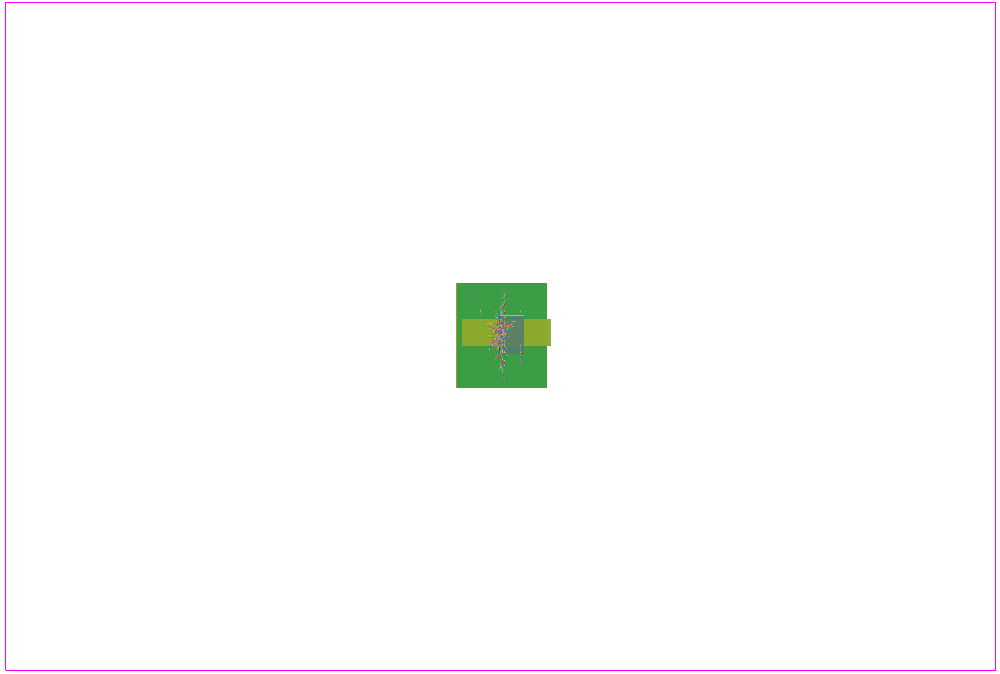
\includegraphics[width=\textwidth]{epsilon/placement_Chip2_100_iterations.png}
  \caption{100 iterations}
 \end{subfigure}
 \hfill
 \begin{subfigure}{.48\textwidth}
  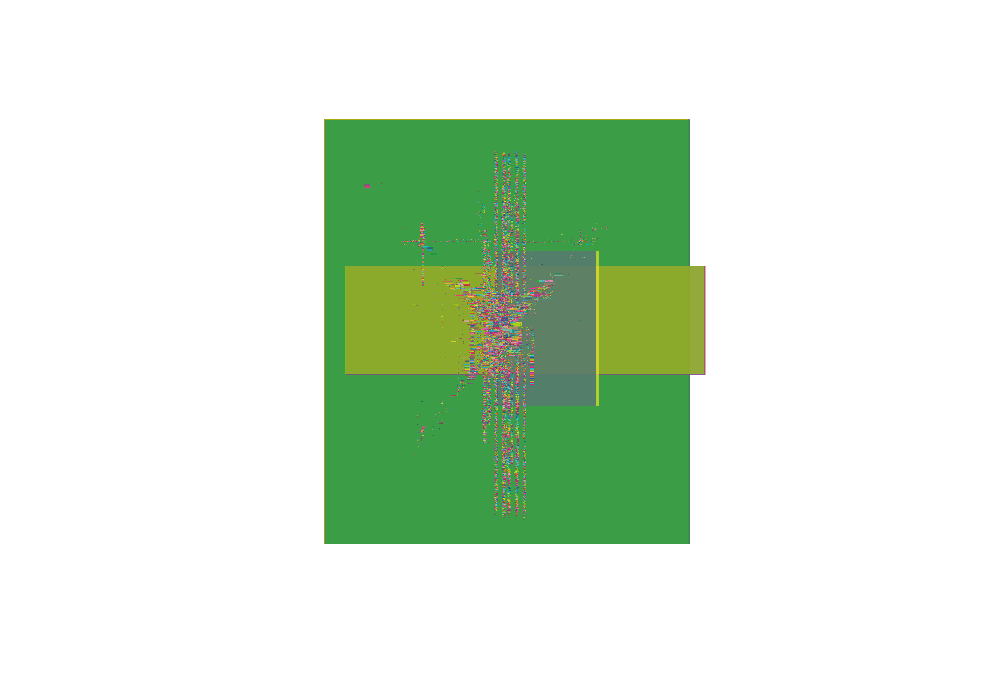
\includegraphics[width=\textwidth, frame]{epsilon/placement_Chip2_100_iterations_zoomed.png}
  \caption{100 iterations, zoomed in on center}
 \end{subfigure}
 
 \bigskip
 
 \begin{subfigure}{.48\textwidth}
  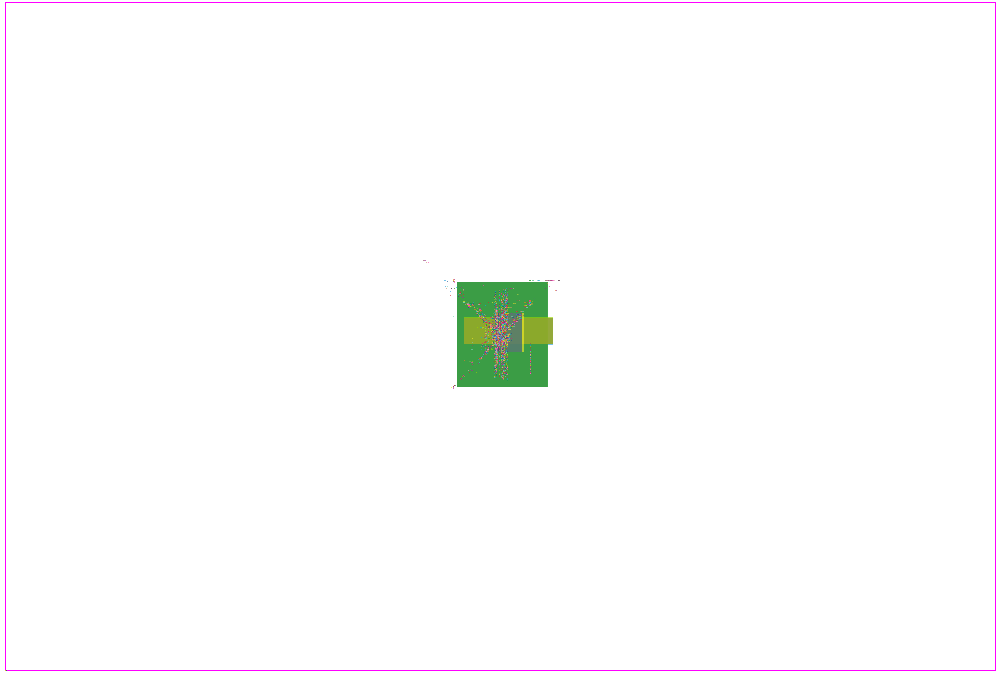
\includegraphics[width=\textwidth]{epsilon/placement_Chip2_200_iterations.png}
  \caption{200 iterations}
 \end{subfigure}
 \hfill
 \begin{subfigure}{.48\textwidth}
  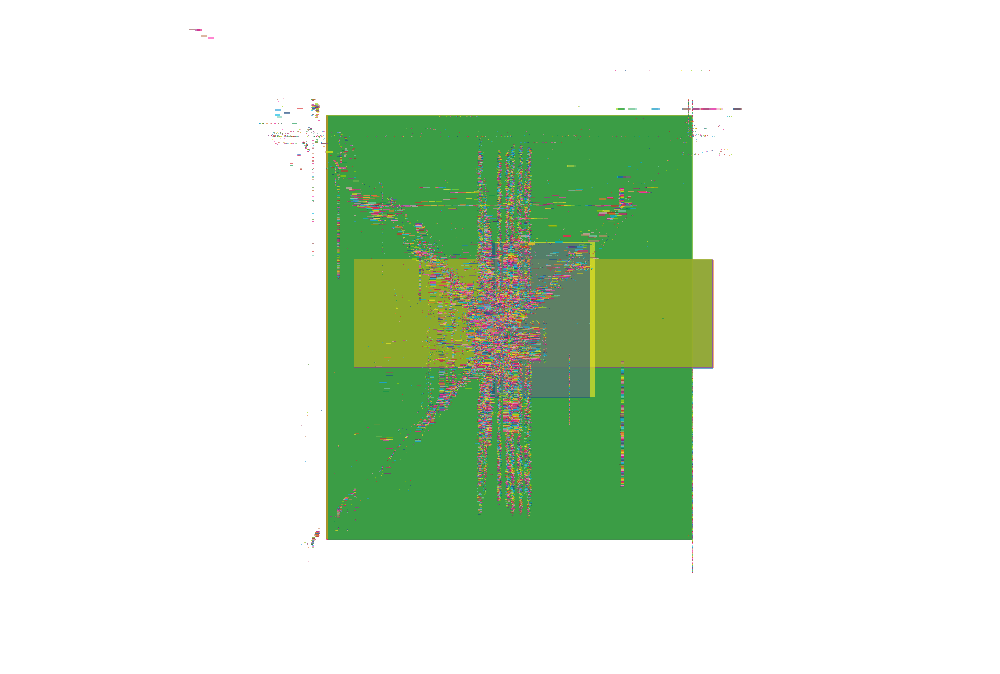
\includegraphics[width=\textwidth, frame]{epsilon/placement_Chip2_200_iterations_zoomed.png}
  \caption{200 iterations, zoomed in on center}
 \end{subfigure}

 \caption{Placement plots after 50, 100 and 200 NAG iterations for \texttt{Chip2}}
 \label{fig:placement_Chip2_depending_on_max_iterations}
\end{figure}

\begin{figure}[p]
 \centering

 \begin{subfigure}{\textwidth}
  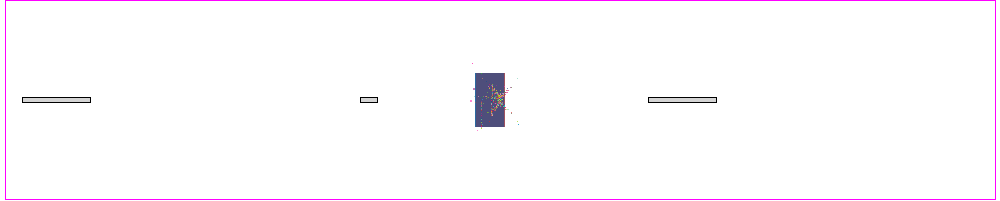
\includegraphics[width=\textwidth]{epsilon/placement_Chip3_50_iterations.png}
  \caption{50 iterations}
 \end{subfigure}
 
 \bigskip
 
 \begin{subfigure}{\textwidth}
  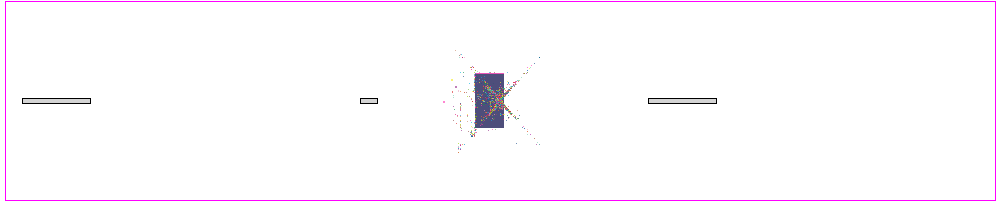
\includegraphics[width=\textwidth]{epsilon/placement_Chip3_100_iterations.png}
  \caption{100 iterations}
 \end{subfigure}
 
 \bigskip
 
 \begin{subfigure}{\textwidth}
  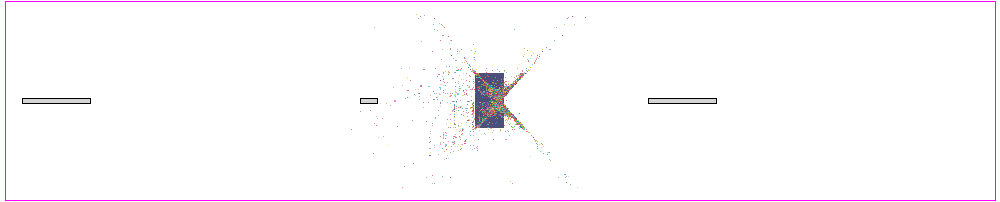
\includegraphics[width=\textwidth]{epsilon/placement_Chip3_200_iterations.png}
  \caption{200 iterations}
 \end{subfigure}

 \caption{Placement plots after 50, 100 and 200 NAG iterations for \texttt{Chip3}}
 \label{fig:placement_Chip3_depending_on_max_iterations}
\end{figure}

\begin{figure}[p]
 \centering

 \begin{subfigure}{0.75\textwidth}
  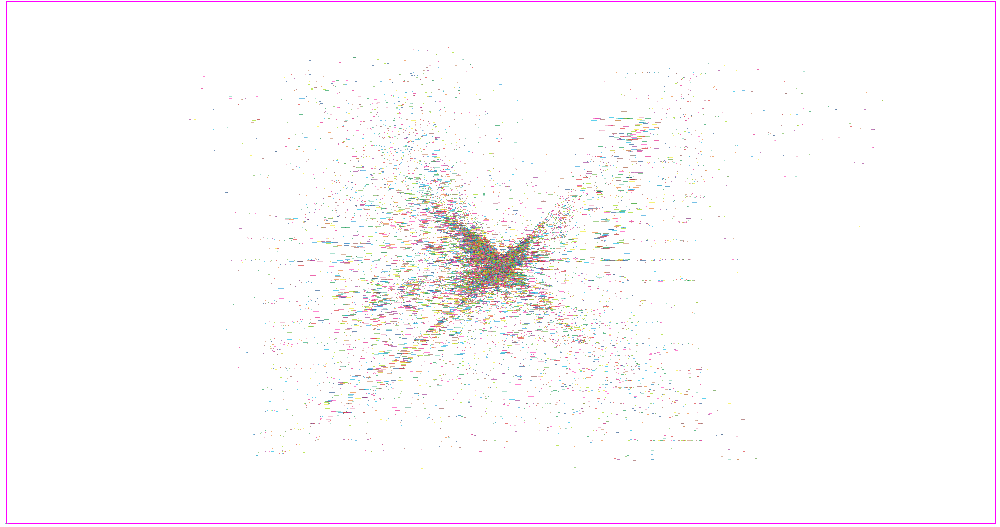
\includegraphics[width=\textwidth]{epsilon/placement_Chip4_50_iterations.png}
  \caption{50 iterations}
 \end{subfigure}
 
 \bigskip
 
 \begin{subfigure}{0.75\textwidth}
  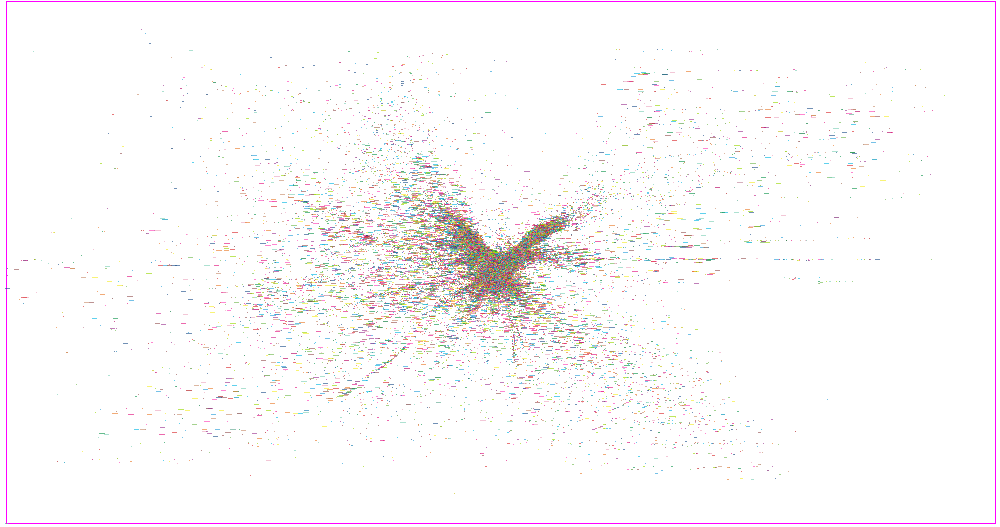
\includegraphics[width=\textwidth]{epsilon/placement_Chip4_100_iterations.png}
  \caption{100 iterations}
 \end{subfigure}
 
 \bigskip
 
 \begin{subfigure}{0.75\textwidth}
  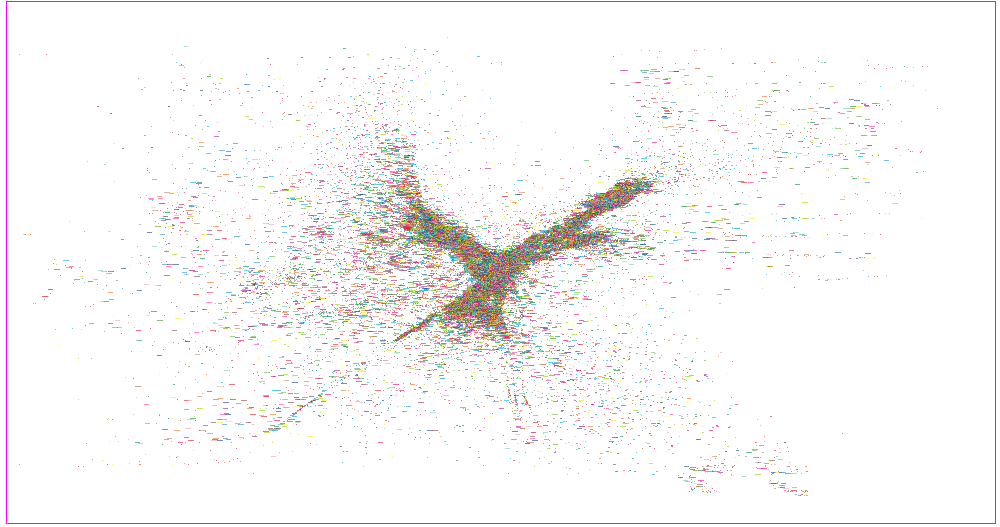
\includegraphics[width=\textwidth]{epsilon/placement_Chip4_200_iterations.png}
  \caption{200 iterations}
 \end{subfigure}

 \caption{Placement plots after 50, 100 and 200 NAG iterations for \texttt{Chip4}}
 \label{fig:placement_Chip4_depending_on_max_iterations}
\end{figure}

\begin{table}[ht] 
 \centering
 \begin{tabular}{c c c c c c}
  Instance       & 50 iterations & 100 iterations   & 200 iterations \\
  \hline
  \texttt{Chip1} & 230.817       & 410.340          & 887.025 \\
  \texttt{Chip2} & 208.221       & 394.730          & 755.941 \\
  \texttt{Chip3} & 82.912        & 167.200          & 311.384 \\
  \texttt{Chip4} & 30.660        & 74.842           & 155.498 \\
 \end{tabular}
 \caption{The runtimes of varying numbers of iterations in seconds}
 \label{table:runtime_depending_on_max_iterations}
\end{table}

It can be seen that there is a huge difference in how much the cells are spreaded
between the large chips and the small chips.
While even 200 iterations do not suffice to move more than a few cells out of the center for \texttt{Chip1} and \texttt{Chip2},
(compare these plots with \cref{fig:baseline_placement_plots})
the situation is much better for \texttt{Chip4} where a good spread can be seen after just 50 iterations.
This can indicate that \(\NWA\) wirelength estimation works better with small chips
and that large chips just need more iterations or that some of the parameters need to be chosen differently for large chips.
It would be interesting to see, for example, whether increasing the \(\gamma\) value further
makes the spreading of cells over the chip area faster.
In this case one could adapt the \(\gamma\) value to the size of the chip.

The runtimes in \cref{table:runtime_depending_on_max_iterations} show that
the runtime increases roughly linearly with the number of iterations.
It is also roughly linear in the number of pins which is as expected because it can be observed
that evaluating the gradient is the most expensive operation of NAG in our case
and evaluating the gradient of \(\NWA\) is done in \(O(\abs{P})\) time (see \cref{sec:theortical_runtimes}).

It is unclear which number of iterations gives us the best compromise between spread and runtime in general
but for the sake of the comparisons with \(\HPWL\) and \(\QCLIQUE\) in the next section
we will perform 200 iterations on each of the chips.
